\documentclass[a4paper,10pt]{article}
\usepackage{polski}
\usepackage[utf8]{inputenc}
\usepackage{array, graphicx}
%custom margins
\usepackage[left=2.5cm, top=2.5cm, bottom=3cm, right=2cm, foot=2cm, head=0.5cm]{geometry}
\usepackage{fancyhdr}
\usepackage[bookmarks=true, pdftex]{hyperref}

%styl nagłowków
\pagestyle{fancy}
\parindent 2cm

%opening
\title{Studium wykonalności}
\author{3@KASK}

\begin{document}
\bibliographystyle{plain}


\maketitle


\begin{center}
%budowanie tabeli
\begin{tabular}{|p{7cm}|p{7cm}|}
\hline
Symbol projektu: & Opiekun projektu:   \tabularnewline
3@KASK & mgr inż. Tomasz Boiński    \tabularnewline \hline
\multicolumn{2}{|l|}{Nazwa Projektu: } \tabularnewline
\multicolumn{2}{|l|}{Wizualizacja grafów za pomocą biblioteki Prefuse } \tabularnewline
\hline
\multicolumn{2}{l}{ } \tabularnewline %pusta linijka
\hline
Nazwa Dokumentu: & Nr wersji:   \tabularnewline
Studium wykonalności & 0.8 \tabularnewline \hline
Odpowiedzialny za dokument: & Data pierwszego sporządzenia:   \tabularnewline
Anna Jaworska & 31.03.09 \tabularnewline \hline
Przeznaczenie: & Data ostatniej aktualizacji:   \tabularnewline
WEWNĘTRZNE & 16.06.09 \tabularnewline \hline
\end{tabular}
\end{center}

\begin{center}
\begin{tabular}{|c|p{4cm}|c|p{3cm}|c|}
\multicolumn{5}{c}{\textbf{Historia dokumentu}} \tabularnewline \hline
\textbf{Wersja} & \textbf{Opis modyfikacji} & \textbf{Rozdział/strona} & \textbf{Autor modyfikacji} & \textbf{Data} \tabularnewline \hline
0.0 & Przygotowanie zarysu dokumentu i określenie zakresu badań & wszystkie & Anna Jaworska & 31.03.09 \tabularnewline \hline
0.1 & Zdefiniowanie wymagań  & 3 & Cały zespół & 31.03.09  \tabularnewline \hline
0.2 & Dołaczenie opisu poprawnego tworzenia bibliotek & 3.5 & Radosław Kleczkowski & 01.04.09\tabularnewline \hline
0.3 & Dołączenie opisów bibliotek graficznych  & 6.2 & Piotr Kunowski & 02.04.09 \tabularnewline \hline
0.4 & Opis uwarunkowań prawnych i rozszerzenie opisu wariantów & 5, 6.1, 7 & Anna Jaworska & 06.04.09\tabularnewline \hline
0.5 & Uzupełnienie braków & wszystkie  & Cały zespół & 07.04.09 \tabularnewline \hline
0.6 & Dołączenie opisu odmian języka OWL i korekta & 6.1, 7  & Piotr Orłowski & 07.04.09 \tabularnewline \hline
0.7 & Korekta & 6.1, 7  & Radosław Kleczkowski i Piotr Orłowski & 15.06.09 \tabularnewline \hline
0.8 & Dołączenie harmonogramów & 8, 9  & Radosław Kleczkowski & 16.06.09 \tabularnewline \hline
\end{tabular}


\end{center}
\newpage
\tableofcontents
\newpage

\section{Założenia realizacji studium}

\subsection{Podstawa wykonania i temat studium}
\paragraph{} Studium wykonywane jest przede wszystkim aby określić możliwe sposoby realizacji projektu. Ma także za zadanie zebranie i podsumowanie informacji potrzebnych zespołowi do realizacji projektu.

\subsection{Cel studium}
\paragraph{} Celem studium jest zbadanie na potrzeby projektu \textit{Wizualizacja grafów za pomocą biblioteki Prefuse}:
\begin{itemize}
 	\item jak należy tworzyć biblioteki w technologii Java
 	\item jakich mechnizmów wizualizacji grafów dostarczają biblioteki Java
	\item czy realizacja projektu za pomocą Prefuse jest odpowiednim rozwiązaniem
	\item jaki standard OWL powinien być wspierany przez wytworzony produkt
\end{itemize}

\subsection{Ograniczenia}
\paragraph{} Do podstawowych ograniczeń należą:
\begin{itemize}
 	\item konieczność realizacji projektu w języku Java
	\item konieczność wykorzystania wersji bibliotek zgodnych z użytymi w OCS
	\item limit czasowy projektu
\end{itemize}



\section{Stan istniejący}

\subsection{Inne systemy i zasoby mające wpływ lub będące pod wypływem planowanego produktu}

\begin{itemize}
 	\item OCS - Ontology Creation System
	\item OWL API ver 2.1.1 - API do przetwarzania plików w formacie OWL zgodnych ze standardem W3C; ta wersja API została użyta w projekcie OCS
	\item biblioteki graficzne - w szczególności Prefuse
\end{itemize}


\subsection{Istniejące na rynku podobne rozwiązania}

\begin{itemize}
 \item Protege - bardzo znany system do edycji i wizualizacji ontologii autorstwa Stanford University. Napisany w języku Java. Ze względu na fakt, iż jest aplikacją standalone, wykorzystującą stosunkowo duże zasoby systemowe i trudną do integracji z portalem OCS, nie może zostać wykorzystana jako gotowe rozwiązanie.

\end{itemize}

\subsection{Problem i motywacja wdrożenia nowego produktu}
\paragraph{} Nowa biblioteka powinna powstać aby:
\begin{itemize}
 \item ułatwić programistom wizualizację ontologii
\item zapewnić API pozwalające na bezpośrednią translację OWL na postać graficzną
\item zapewnić rozwiązane przenośnie i uniwersalne
\end{itemize}



\section{Ogólne wymagania stawiane produktowi i ich priorytety}
\paragraph{} Wymienione wymagania mają charakter orientacyjny, pozwalający nakreślić zakres problemu jaki ma pokrywać projekt. Szczegółową definicję wymagań będzie zawierać dokument \textit{Specyfikacji wymagań}. W szczególność możliwe jest, że niektóre z wymienionych poniżej wymagań zostaną usunięte lub zmienione oraz to, że mogą zostać dodane inne wymagania.

\subsection{Użytkownicy}
\paragraph{} Użytkownikami biblioteki będą programiści tworzący aplikacje wizualizujące ontologie. Inicjalnie będą to programiści związani z projektem OCS, później mogą to być dowolni inni programiści chętni do korzystania z biblioteki.
\subsection{Dane}

\paragraph{Obsługiwane formaty} 
Biblioteka powinna obsługiwać te same formaty danych co OWL API (zgodne ze specyfikacją W3C):
\begin{itemize}
 	\item RDF
	\item RDF Schema
	\item OWL Lite
	\item OWL DL
	\item OWL Full
\end{itemize}

\paragraph{Wczytywanie danych}Ponadto dane te powinny być przekazywane poprzez obiekt OWL API.

\paragraph{Modyfikowalność danych} Biblioteka powinna udostępniać metody do modyfikacji wczytanych danych i możliwość zapisania zmienionych danych. Dane powinny być dostarczane użytkownikowi w postaci obietków OWL API. Biblioteka nie musi sprawdzać czy zmiany wprowadzone przez użytkownika są logicznie poprawne.

\subsection{Funkcjonalność}
% tu mozna o OWL napisać i pare innych
\paragraph{} Zakładamy, że biblioteka będzie zawierać następujące funkcjonalności:
\begin{itemize}
 	\item wizualizacja elmentów OWL
	\item definiowanie przez użytkownika własnych akcji dla zdarzeń okna (np. klinięcie, przeciągnięcie wierzchołka grafu)
	\item standardowe definicje zdarzeń okna
	\item wczytywanie, modyfikowanie i zapis ontologi
	\item definiowanie parametrów wyglądu, w szczególności ilości widocznych poziomów grafu
\end{itemize}



\subsection[Wymogi techniczno - technologiczne]{Wymogi techniczno - technologiczne: Standard tworzenia biblioteki }
%tu beda radkowe zalecenia


\paragraph{} Nie istnieją żadne formalne zalecenia dotyczące tworzenia bibliotek JAVA. Są jednak pewne zalecenia co do stosowanych praktyk \footnote{Greg    Travis.          Build    your   own     java  library.          publikacja
\url{http://www.digilife.be/quickreferences/PT/Build your own Java library.pdf}.
}:
\begin{enumerate}
\item \textbf{Odpowiednie kapsułkowanie.} Publiczne powinny być jedynie te klasy i metody, które są istotne dla użytkownika i z których będzie on bezpośrednio korzystał.
\item \textbf{Możliwość debugowania.} Użytkownik powinien mieć możliwość debugowania kodu biblioteki, bez konieczności znajomości każdego jej szczegółu.
\item  \textbf{Przejrzystość.} Kod biblioteki powinien być odpowiednio udokumentowany za pomocą javadoc. W szczególności, bardzo dokładnie należy opisać klasy oraz metody publiczne.
\item \textbf{Łatwość użycia.} Biblioteka powinna zawierać klasy, pokazujące przykłady wykorzystania jej klas i metod.
\item \textbf{ Rozszerzalność.} Struktura wewnętrzna biblioteki powinna być odpowiednio podzielona na klasy (wykorzystując klasy abstrakcyjne i interfejsy. Dzięki temu użytkownik będzie miał możliwość stworzenia własnych klas, rozszerzających funkcjonalność biblioteki.
\item \textbf{Uniwersalność.} Biblioteka powinna mieć jasno określony problem, który rozwiązuje. Wyniki powinny być podane użytkownikowi w wygodny dla niego sposób (lub na kilka sposobów), który będzie umożliwiał wykorzystanie biblioteki w różnych aplikacjach. Innymi słowy, biblioteka powinna udostępniać łatwy i przejrzysty dla użytkownika interfejs.
\item Biblioteka powinna być napisana w taki sposób, aby użytkownik spojrzał na nią i mógł powiedzieć: "Wow, to jest dokładnie to, czego potrzebuję i dokładnie tak samo bym to napisał!".

\end{enumerate}



\section{Ogólna ocena ryzyka i planowany sposób zarządzania nim}


\paragraph{Schemat opisu czynnika ryzyka}
\begin{center}
\begin{tabular}{|l|p{12cm}|}
\hline
\textbf{ID czynnika} &  RISKXX \tabularnewline \hline
\textbf{Nazwa czynnika} & Nazwa \tabularnewline \hline
\textbf{Opis czynnika} & Opis... \tabularnewline \hline
\textbf{Sposób zarządzania} & Opis.. \tabularnewline \hline
\end{tabular}
\end{center}

\subsection{Czynniki ryzyka}
\begin{center}
\begin{tabular}{|l|p{12cm}|}
\hline
\textbf{ID czynnika} &  RISK01 \tabularnewline \hline
\textbf{Nazwa czynnika} & Problemy logistyczne zespołu  \tabularnewline \hline
\textbf{Opis czynnika} & Uwzględniamy możliwość wystąpienia problemów osobistych członków zespołu powodujących ich wyłączenie z prac. \tabularnewline \hline
\textbf{Sposób zarządzania} & Jeśli ktoś zostanie wyłączony z prac, reszta zespołu musi podzielić między siebie jego obowiązki i informować osobę wyłączoną o postępach, tak aby ona miała wgląd w postęp prac, które miała wykonywać i kontynuować je po niedyspozycji.  \tabularnewline \hline
\end{tabular}
\end{center}


\begin{center}
\begin{tabular}{|l|p{12cm}|}
\hline
\textbf{ID czynnika} &  RISK02 \tabularnewline \hline
\textbf{Nazwa czynnika} & Problemy członków zespołu na uczelni \tabularnewline \hline
\textbf{Opis czynnika} & Możliwe jest powstanie zaległości związanych z innymi uczelnianymi obowiązkami    \tabularnewline \hline
\textbf{Sposób zarządzania} & Członek zespołu musi zgłosić swoje problemy reszcie zespołu. W zależności od sytuacji termin wykonania jego zadań zostanie przedłużony lub zadania te przejmie ktoś inny. \tabularnewline \hline
\end{tabular}
\end{center}

\begin{center}
\begin{tabular}{|l|p{12cm}|}
\hline
\textbf{ID czynnika} &  RISK03 \tabularnewline \hline
\textbf{Nazwa czynnika} & Niedostępność opiekuna/klienta \tabularnewline \hline
\textbf{Opis czynnika} & Z różnych przyczyn niezależnych od zespołu opiekun może stać się niedostępny.  \tabularnewline \hline
\textbf{Sposób zarządzania} & Wszelkie problemy wymagające, według zespołu, poznania opinii opiekuna będą musiały zostać rozwiązanie poprzez podjęcie decyzji przez zespół bez wsparcia. Wszelkie problemy organizacyjne związane z projektem grupowym powinny być pod nieobecność opiekuna zgłaszane do katedralnego koordynatora projektów grupowych.     \tabularnewline \hline
\end{tabular}
\end{center}


\begin{center}
\begin{tabular}{|l|p{12cm}|}
\hline
\textbf{ID czynnika} &  RISK04 \tabularnewline \hline
\textbf{Nazwa czynnika} & Niewystarczająca wiedza programisty \tabularnewline \hline
\textbf{Opis czynnika} & W trakcie pisania kodu może okazać się, że programista z powodu nieznajomości bibliotek/metod/praktyk zacznie mieć problemy z wydajnym kodowaniem (zacznie popełniać częste błędy, pracować bardzo wolno).  \tabularnewline \hline
\textbf{Sposób zarządzania} & Osoba mająca problemy z danym kodem powinna zgłosić to reszcie zespołu. Jeśli ograniczenia czasowe na to pozwolą dostanie ona dodatkowy czas na wykonanie zadania. Jeśli nie będzie to możliwe, zadanie zostanie przekazanie osobie będącej w stanie poradzić sobie z zagadnieniem lub zostanie podzielone między większą liczbę osób. \tabularnewline \hline
\end{tabular}
\end{center}

\begin{center}
\begin{tabular}{|l|p{12cm}|}
\hline
\textbf{ID czynnika} &  RISK05 \tabularnewline \hline
\textbf{Nazwa czynnika} & Awaria SVN \tabularnewline \hline
\textbf{Opis czynnika} & Serwer SVN nie jest dostępny lub działa w sposób nieporządany. \tabularnewline \hline
\textbf{Sposób zarządzania} & Problem należy niezwłocznie zgłosić opiekunowi i oczekiwac na jego interwencję. \tabularnewline \hline
\end{tabular}
\end{center}



\section{Uwarunkowania prawne i inne}
%na jakiej to ma byc licencji - tylko dla KASK-u ?
\paragraph{} Docelowy produkt będzie własnością Katedry Architektury Systemów Komputerowych wydziału Elektroniki, Telekomunikacji i Informatyki Politechniki Gdańskiej.  Należy zadbać  o to aby używane w projekcie biblioteki były na licencjach pozwalających na użycie w produkcie zamkniętym.


\section{Proponowane rozwiązania}

\paragraph{} Proponowane rozwiązania zostaną rozważone pod względem wersji OWL oraz biblioteki graficznej.

%wariant z DL
%wariant z Full
%wybór w dizedzinach - biblioteki i Java - wersje itp, wersja OWL(RDF?), wersja standardu tworzenia biblioteki, wzorować się na cyzms istniejącym (?)
\subsection{Wersja OWL}

\begin{description}
 \item[Lite]
 \begin{itemize}
	 \item zawiera bazowe elementy OWL i RDF
		\begin{itemize}
 		\item typy: Class, Property, Individual
		\item podstawowe nierówności, zależności, charakterystyki
		\item elementarna kardynalność
		\item adnotacje
		\end{itemize}
	\item pozwala budować hierarchię elementów
	\item wymaga separacji typów
	\end{itemize}
\item[DL]
\begin{itemize}
	\item zawiera wszystkie elementy języka OWL Lite
	\item dodatkowo zawiera zaawansowane elementy języka OWL
		\begin{itemize}
 		\item ma rozwiniętą obsługe zależności między elementami podstawowymi
		\item obsługuje kardynalność w jej pełnej formie
		\end{itemize}
	\item można go bezpośrednio mapować na logikę opisową SHOIN - jest rozstrzygalny
	\item tą wersję obsługuje portalSubsystem
	\end{itemize}
\item[DL]
\begin{itemize}
	\item zawiera wszystkie elementy OWL DL
	\item nie wymaga separacji typów
	\item ma mniejsze ograniczenia od OWL DL
	\item nie ma w nim gwarancji rozstrzygalności dla wnioskowań
	\end{itemize}
\item[Full]
 
\end{description}

\paragraph{} Należy zwrócić uwagę, że specyfikacja OWL jest dobrze zdefiniowana (rekomendacja W3C\footnote{Frank van Harmelen Deborah L. McGuinness. Owl web ontology language overview. publikacja elektroniczna, luty 2004.\url{http://www.w3.org/TR/2004/REC-owl-features-20040210/}
}) co sprawia, że zachodzi spójność pomiędzy jej elementami. Zaimplementowanie wersji bardziej rozwiniętej oznacza, że wymogi dla wersji niższej także zostaną spełnione.




	


	

	



\subsection{Proponowane biblioteki do wizualizacji grafów}


\begin{description}
\item[Prefuse]
 jest elastycznym pakietem dostarczającym programiście narzędzia do przechowywania danych, manipulowania nimi oraz ich interaktywnej wizualizacji. Biblioteka jest rozwijana w całości w języku Java. Może być wykorzystana do budowania niezależnych aplikacji, wizualnych komponentów rozbudowanych aplikacji oraz tworzenia apletów.


Podstawowe cechy i elementy:
\begin{itemize}
\item kilkadziesiąt algorytmów i metod wizualizacji danych m.in: ForceDirectedLayout, RadialTreeLayout, NodeLinkTreeLayout, SquarifiedTreeMapLayout
\item dynamiczne rozmieszczanie i animacje
\item transformacje, przekształcenia geometryczne oraz przybliżanie/oddalanie obrazu
\item podstawowym elementem struktury danych jest krotka
\item krotki mogą być tworzone bezpośrednio w aplikacji lub na podstawie zewnętrznych danych
\item wbudowany język zapytań do filtrowania danych
\item tworzenie struktur danych na podstawie zewnętrznych plików (CSV, XML) oraz bazy danych
\item klasy wspomagające synchronizację danych pomiędzy tabelami Prefuse a bazą danych
\item Prefuse posiada licencję BSD
\end{itemize}

 \item[Piccolo]  


 jest zastawem narzędzi używanych przy tworzeniu graficznych aplikacji. Często wykorzystywana do tworzenie interfejsów użytkownika. w których elementy są przybliżane i oddalane. Istnieją trzy wersje tej biblioteki: Piccolo.Java, Piccolo.NET oraz PocketPiccolo.NET. Posiada Licencje BSD.
\item[JUNG (Java Universal Network/Graph Framework)]

 Biblioteka przeznaczona do wizualizacji danych za pomocą grafów oraz sieci. Umożliwia wizualizację nie tylko grafów prostych, ale m.in. multigrafów, digrafów oraz grafów posiadających wagi i etykiety na wierzchołkach i krawędziach. Biblioteka posiada podstawowe algorytmy grafowe. Została napisana w całości w Javie i wydana na licencji BSD.
\item[JGraph]

 Napisana w pełni w Javie biblioteka do wizualizacji grafów kompatybilna ze Swingiem. Posiada wiele ciekawych opcji wizualizacji zarówno wierzchołków jak i krawędzi grafów. Poza algorytmami wizualizacji w jej skład wchodzą podstawowe algorytmy grafowe. Została wydana na licencji LGPL.
\end{description}



\section{Rekomendowany wariant}


\paragraph{OWL:} 
 Po zapoznaniu się ze specyfikacją stworzoną przez W3C najbardziej sensownym wydaje się być wykorzystanie wersji DL języka OWL. Dodatkowo wersja ta była dotychczas wykorzystywana przez portalSubsystem. Grupa nie odrzuca możliwości zaimplementowania obsługi wersji OWL Full, która pod względem zawartych w niej elementów zasadniczo nie różni się od wersji DL. Na jej niekorzyść przemawia jednak argument w postaci tego, że umożliwia pewne niejasności w prezentacji (szczególnie pod względem rozróżniania typów).

\paragraph{Biblioteka:}

Po uważnym przejrzeniu bibliotek najbardziej użyteczne wydają się Prefuse oraz Piccolo. Ze względu na dostępność dużej ilości przykładowego kodu wykorzystującego Prefuse w portalSubsystem wykorzystana zostanie biblioteka Prefuse. Ponadto opinie wyrażone w pracy magisterskiej Andrzeja Jakowskiego silnie przemawiają na korzyść Prefuse.


\section{Strategia i wstępny harmonogram}

\paragraph{} Ze względu na doświadczenie zespołu z Rational Unified Process (trzej członkowie zespołu uprzednio zrealizowali projekt w tej metodyce), zostanie on zastosowany z uwzględnieniem stosowanych dla charakteru projektu modyfikacji, w szczególności:
\begin{itemize}
 \item celem projektu jest wytworzenie biblioteki, więc nie pojawią się typowe diagramy warstwy danych
\item model interfejsu graficznego zostanie zastąpiony modelem interfejsów/funkcjonalności zewnętrznych udostępnianych przez pakiety i/lub klasy
\item modele dynamiki zostaną okrojone do ilości faktycznie potrzebnej programistom
\end{itemize}
\paragraph{}Pomimo ustalenia harmonogramu z terminami oddania dokumentów należy wziąć pod uwagę charakter metodyki RUP, która zakłada przyrostowe wytwarzanie dokumentacji - w póżniejszych etapach projektu pojawią się zmodyfikowane wersje wytorzonych wcześniej dokumentów.

\subsection{Harmonogram na I semestr}
\begin{center}
 \scalebox{0.45}{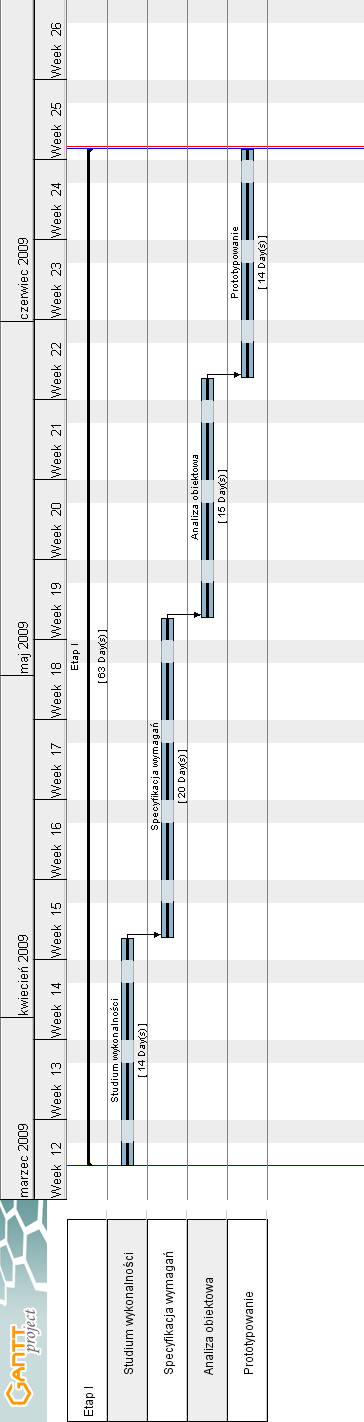
\includegraphics{./elementyGraficzne/harmonogramy/sem1.png}}\end{center}
\subsection{Harmonogram na II semestr}
\begin{center}
 \scalebox{0.5}{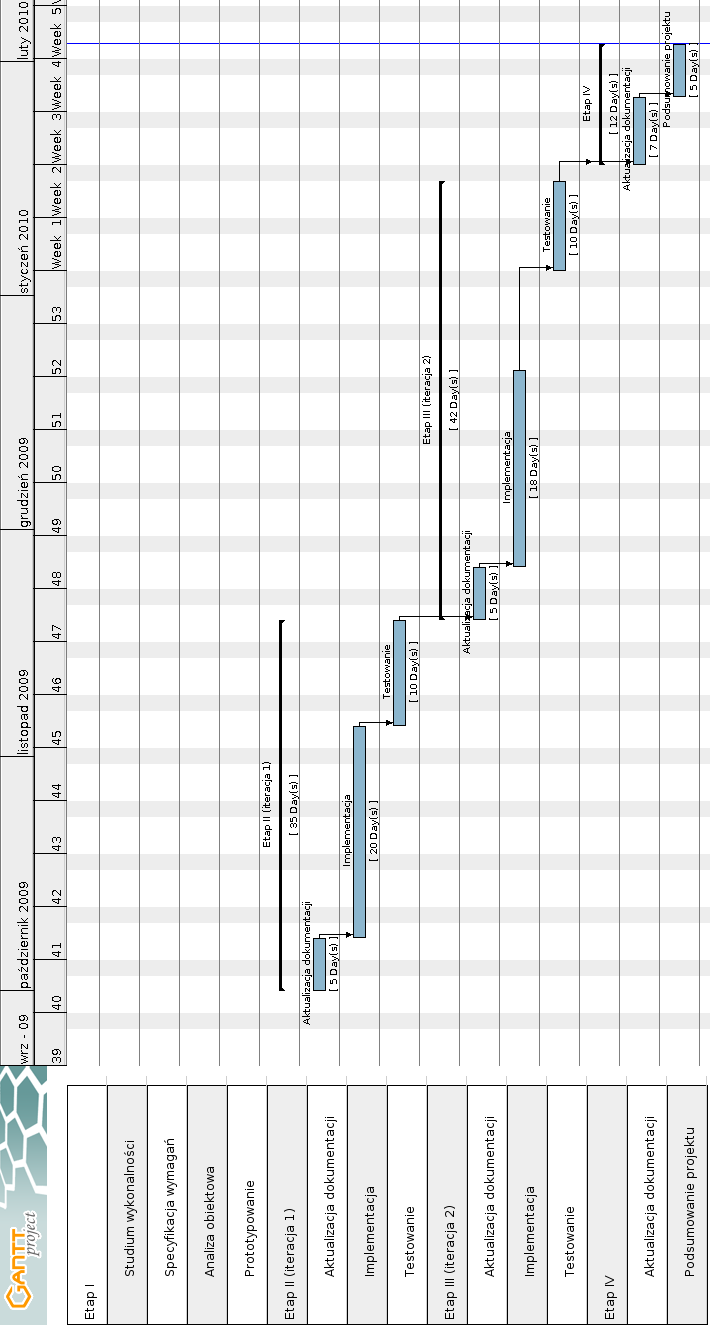
\includegraphics{./elementyGraficzne/harmonogramy/sem2.png}}\end{center}






%\clearpage
%\phantomsection
%\addcontentsline{toc}{section}{Literatura}
%\bibliography{biblio}

\end{document}
